This layer is the most fragile yet the most critical aspect of our application. This is where the information from the user is stored so that it can be accessed when required in future. We will be using subsytem such as Firebase, SQLite and Global barcode inventory. This layer will be the fulcrum to our team creating and effective management system. Multiple information will be recorded in this layer. This includes login credentials, a product’s name, flavor, type and so on. In brief, this layer will execute the query given by the user in presentation layer and process the result back to application layer which will finally process the information to be displayed in the presentation layer.

\subsection{Firebase}
Firebase is Google's mobile platform a cloud-hosed database where data is stored as JSON and is synchronized in the realtime. Beverage Management will be build on the Android OS, all of our client will share one Realtime Database instance and will receive updates with the newest data.

This subsystem will be our main component, it will store and retrieve the user's access credentials, will engage with Database connectivity of the application layer, and SQLite subsystem to store and retrieve data locally. 

\begin{figure}[h!]
	\centering
 	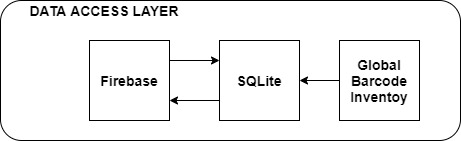
\includegraphics[width=0.60\textwidth]{images/DS.jpg}
 \caption{Example subsystem description diagram}
\end{figure}

\subsubsection{Assumptions}
We are going to assume that the:
\begin{itemize}
    \item The connection with Application layer will be made successfully via Database Connectivity to initiate the firebase. 
    \item The connection between Firebase and the SQLite is established successfully. 
\end{itemize}

\subsubsection{Responsibilities}
This subsystem will be responsible to process the access to the SQLite information if the credentials are correct.

\subsubsection{Subsystem Interfaces}
\begin {table}[H]
\caption {Firebase interfaces} 
\begin{center}
    \begin{tabular}{ | p{1cm} | p{6cm} | p{3cm} | p{3cm} |}
    \hline
    ID & Description & Inputs & Outputs \\ \hline
    \#1 & Firebase will have direct relation with the application layer. & Takes credentials information as a input  & Gives access rights as an output to the SQLite. \\ \hline
    \end{tabular}
\end{center}
\end{table}


\subsection{SQLite}
SQLite is a programming library which implements a relational database management system. The SQLite database concept is, in contrast to other client-server systems, to be linked into the applications code, instead of providing a standalone daemon with which an application can communicate to request or write data. Because of the small size of the library itself, and the ease of use, it is esepcially interesting for embedded systems. SQLite supports a variety of SQL-  (Structured Query Language) commands with some exceptions and does not provide any access or user-management. That means, that everyone, who can access the database file, can access the data as well as write (change, delete, add) data, if he can write the database file. It therefore inherits the access permissions of the filesystem. 

\begin{figure}[h!]
	\centering
 	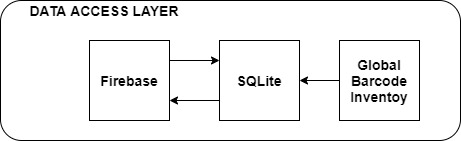
\includegraphics[width=0.60\textwidth]{images/DS.jpg}
 \caption{Example subsystem description diagram for SQLite}
\end{figure}

\subsubsection{Assumptions}
We are going to assume that we will be reading and writing data to the SQLite as a local database at this moment.

\subsubsection{Responsibilities}
This subsystem will be responsible to process the information that will be stored in the database locally and the application layer can access the information. 

\subsubsection{Subsystem Interfaces}
\begin {table}[H]
\caption {SQLite interfaces} 
\begin{center}
    \begin{tabular}{ | p{1cm} | p{6cm} | p{3cm} | p{3cm} |}
    \hline
    ID & Description & Inputs & Outputs \\ \hline
    \#1 & SQLite will communicate via Firebase subsystem component and directly from Data Access Query. & Takes instruction from Application layer in the form of queries. & Gives the appropriate response to the instruction provided to the Java Application layer.\\ \hline
    \#2 & SQLite will also intended to communicate with Global Barcode Inventory subsystem component. & Takes the response from Global Barcode Inventory. & Gives the appropriate response to the instruction provided to the Java Application layer.\\ \hline
    \end{tabular}
\end{center}
\end{table}

\subsection{Global Barcode Inventory}
Barcodes are symbols that can be scanned electronically using laser or camera-based systems. They are used to encode information such as product numbers, serial numbers and batch numbers. We will be using some third party global barcode inventory that will provide us with all beverages in the industry.

\begin{figure}[h!]
	\centering
 	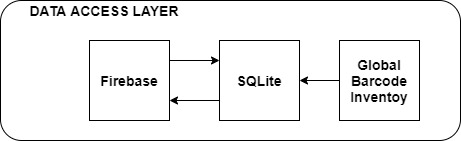
\includegraphics[width=0.60\textwidth]{images/DS.jpg}
 \caption{Example subsystem description diagram for Global Barcode Inventory}
\end{figure}

\subsubsection{Assumptions}
We are going to assume that the inventory are accurate.

\subsubsection{Responsibilities}
This subsystem will be responsible to process the product information in the industry currently. 

\subsubsection{Subsystem Interfaces}
\begin {table}[H]
\caption {Global Barcode Inventory interfaces} 
\begin{center}
    \begin{tabular}{ | p{1cm} | p{6cm} | p{3cm} | p{3cm} |}
    \hline
    ID & Description & Inputs & Outputs \\ \hline
    \#1 & SQLite will access the prodiuct information form the inventory subsystem. & Takes instruction from Application layer in the form of queries. & Gives the appropriate response to the SQLite and will to the Application layer.\\ \hline
    \end{tabular}
\end{center}
\end{table}

